\section{Stage 4: rules, rosters and configurations}
\label{app:stage4}

S4.1--S4.3 and both discovery and held-out evaluation of the revised final
S4.4 experiment (S45 in the implementation) have been executed. The latter
replaces the earlier S4.4--S4.5 retention/reduction design. The design is in
Appendix~\ref{app:final-ri}; discovery results and frozen 87-family validation
are reported separately below with their actual populations.

\paragraph{Route semantics.}
The source's pre-projection slice $z=AV$ is replaced by the donor value; the shared
attention-output normalization stays live; all other residual-branch increments
between source and receiver are frozen after their normalization in the hybrid run.
The receiver's channel is recaptured from the hybrid residual and injected into a
fresh recipient run: for fact-site K/V routes at the fact positions, with only the
receiver's original colon output row released; for Q routes at the colon. In the
recipient run all later computation is live. A retained route supports transmission
through the declared source, site and receiver channel in this frozen background;
its effect is not an additive share of the source's full-model importance.
Separately measured routes do not establish their composition into a chain.
Effects are averaged over orders
within family and then over families; 20,000-draw family-bootstrap intervals are
descriptive after selection. \emph{Retention rule}, fixed in advance with
$\tau=0.10$ logits: coherent if $|\bar I|\ge\tau$ with the same sign in at least
70\% of families; heterogeneous if $\mathbb{E}_f|I_f|\ge\tau$ and $|I_f|\ge\tau$ in
at least 20\% of families. The rule orders measurements; it is not a significance
test.

\paragraph{S4.1 sources, receivers, controls.}
Sources with fact-site masks: L17H1 (query-fact mother tokens, ``is'', period, and
their union), L15H25 (child-last, query sentence), L13H10 and L17H3 (sentence
masks), and two coverage candidates outside the inventory, L13H18 and L24H19,
added after a coverage check of the exact common-subset map. Colon sources: the
strong answer-position heads. Receivers are a bounded candidate list built from the
Stage-3 attention profiles and coverage rules, not every later head: for fact-site
sources, later heads attending to the site, channels K and V; for colon sources,
later heads on Q and a residual bypass that tests whether the source's write reaches
the answer without passing through a tested head. Initial measurement on the 40
common pairs; retained routes extended to all 178 pairs in both donor directions
under a cap of 96 extended configurations. Controls by intervention type: random
receivers for head routes; wrong-site masks for fact-site routes; self patches;
reverse-direction routes; the ordinary single-head patch as comparator; order and
prefix sensitivity per route. Counts of retained routes are reported with the
results.

\paragraph{S4.2 groups.}
\begin{center}\small
\begin{tabular}{@{}llp{5.4cm}@{}}
\toprule
ID & Source / site & Members (all replaced at the colon) \\
\midrule
O1 & L13H10 / sentence & L16H1, L17H3, L18H18, L18H19 \\
O2 & L15H25 / child-last & L16H1, L16H21 \\
O3 & L17H1 / mother & L18H18, L18H19, L18H24, L19H16, L20H1, L22H5, L27H6 \\
O4 & L17H3 / colon & L18H18, L18H19 \\
I1 & L27H6 / Q & L18H18, L18H19, L19H16, L20H1, L23H15, L25H17 \\
I2 & L21H23 / KV & L17H24, L18H18, L18H19, L19H16, L20H1 \\
I3 & L30H18 / Q & L18H18, L18H19, L20H1, L23H15, L25H17 \\
I4 & L18H18 / Q & L16H1, L16H21, L17H3 \\
\bottomrule
\end{tabular}
\end{center}
Outgoing groups (O) collect the receivers of one source; incoming groups (I) the
sources of one receiver. With $I(S)$ the importance under simultaneous replacement
of group $S$, whole-group, singleton and group-minus-member patches give
\begin{align*}
N(S)&=I(S)-\sum_{h\in S}I(h),\\
\delta_h(S)&=I(S)-I(S\setminus\{h\}).
\end{align*}
$N(S)$ measures nonadditivity and $\delta_h(S)$ the member's contribution
conditional on the other group members being replaced. Singles, whole groups and group-minus-one masks
deduplicate to 49 base masks under a 128-configuration cap; selected group
contrasts and two blocking contrasts were extended to all 89 families. Receiver
blocking: L17H1's clean activation restored in the corrupted run at its source
masks with the O3 members clamped to their corrupted colon outputs; L15H25 restored
with the O2 pair clamped; self-clamp and reverse controls. The loss of source
restoration under receiver clamping measures dependence on receiver response;
overlapping paths and interactions prevent an exclusive partition into mediation
shares. Mean-replacement
sensitivity was run for the extended contrasts, not for every configuration.

\paragraph{S4.2 RI participation.}
RI31: the RI-selected heads retained by the rule ``best original RI rank $\le3$ in
any ranking, or $\max(|I_h|,|I^F_h|)\ge0.1$'' (23 by rank, 8 by effect). It
contains the eight strong RI heads (positive: L16H1, L16H21, L17H24, L18H19, L22H5;
negative: L19H16, L23H15, L26H23) and 23 residual heads. Reference cohorts: four
sets of 23 non-selected heads matched to the residual set in size and layer
composition; they are compared with the residual 23, not with all 31. Weakened
background $K$: the smallest prefix of the strongest colon readers whose replacement
leaves the symmetric clean-minus-corrupted gap inside a pre-specified range, with a
fallback rule if no prefix qualifies; the rule selected $K=\{$L21H18$\}$ (66\% of the
gap left). All 31 candidates were measured on the common panel; 14 were extended
(the eight strong heads and six retained conditional candidates: L6H24, L8H15,
L14H23, L15H3, L16H31, L20H7). Means are indexed by head, fact slot, token role and
within-name bucket, computed over the 89 families with the evaluated family
excluded. Backup test: L26H31, a name mover with negligible standalone effect, in
five backgrounds with upstream or downstream members replaced; the same retention
rule applies.

\paragraph{S4.1 results: retained routes.}
Of the 96 configurations extended to all 89 families, 95 retain under noising and 93
under restoration; 94 and 92 retain on the additional 69 families alone, and all 96
mean signs agree between the two donor directions (Figure~\ref{fig:routes-app}a).
Table~\ref{tab:routes-app} lists the main retained routes. All 55 controls are smaller
than their target in mean absolute family effect (Figure~\ref{fig:routes-app}b); 7 of
17 other-site controls nevertheless retain under the rule, and 0 of 38 random
receivers. Controls are not norm-matched. Nineteen retained core configurations were
not extended (cap), and L13H18 has no retained route among 138 localized direct
configurations.

\begin{figure}[h]
\centering
\includegraphics[width=\columnwidth]{figH_routes}
\caption{Route mapping on the 89 discovery families. (a) Noising against restoration
effect of the 96 extended configurations, by receiver type. (b) Mean absolute family
effect of each control against that of its target route (log axes); every control lies
below the diagonal.}
\label{fig:routes-app}
\end{figure}

\begin{table}[h]
\centering\scriptsize
\setlength{\tabcolsep}{3pt}
\begin{tabular}{@{}llrrr@{}}
\toprule
Source / site & Receiver / channel & $I_{89}$ & $J_{89}$ & $I_{69}$ \\
\midrule
L17H1 / union & L18H18 / V & $+3.400$ & $+3.335$ & $+3.391$ \\
L17H1 / union & L18H19 / V & $+2.074$ & $+2.054$ & $+2.057$ \\
L17H1 / union & L18H24 / V & $-1.004$ & $-1.070$ & $-0.988$ \\
L17H1 / union & L22H5 / V & $+0.898$ & $+0.865$ & $+0.882$ \\
L17H1 / union & L20H1 / V & $-0.582$ & $-0.576$ & $-0.567$ \\
L17H1 / union & L19H16 / V & $-0.247$ & $-0.225$ & $-0.243$ \\
L15H25 / child-last & L16H1 / V & $+0.182$ & $+0.187$ & $+0.182$ \\
L15H25 / child-last & L16H21 / V & $+0.210$ & $+0.223$ & $+0.215$ \\
L16H1 / colon & L18H18 / Q & $+0.372$ & $+0.370$ & $+0.367$ \\
L16H21 / colon & L18H18 / Q & $+0.349$ & $+0.407$ & $+0.348$ \\
L18H18 / colon & L27H6 / Q & $+0.662$ & $+0.663$ & $+0.674$ \\
L18H19 / colon & L27H6 / Q & $+0.731$ & $+0.742$ & $+0.736$ \\
L13H10 / sentence & L16H1 / V & $-0.175$ & $-0.175$ & $-0.172$ \\
L13H10 / sentence & L17H3 / V & $+0.150$ & $+0.139$ & $+0.151$ \\
L14H26 / sentence & L16H1 / V & $+0.136$ & $+0.140$ & $+0.139$ \\
L17H3 / colon & L18H18 / Q & $-0.158$ & $-0.172$ & $-0.155$ \\
L18H19 / colon & MLP 19 & $+0.532$ & $+0.554$ & $+0.514$ \\
L18H19 / colon & bypass & $+0.754$ & $+0.770$ & $+0.748$ \\
L18H18 / colon & bypass & $+0.547$ & $+0.562$ & $+0.546$ \\
L24H19 / colon & bypass & $+0.165$ & $+0.165$ & $+0.160$ \\
\bottomrule
\end{tabular}
\caption{Main retained routes: noising ($I$) and restoration ($J$) effects on the 89
discovery families and noising on the additional 69 families outside the common
subset. ``Union'' is the union of L17H1's mother-token, ``is'' and period masks;
``bypass'' tests the source's write reaching the answer without passing through a
tested head.}
\label{tab:routes-app}
\end{table}

\paragraph{S4.2 results: blocking, RI participation, backup.}
Table~\ref{tab:blocking-app} gives the receiver-blocking results and
Table~\ref{tab:ri31-app} the RI-participation audit for the 14 extended candidates.
The whole-group effects of the eight G1 groups overlap heavily because the
L18H18/L18H19 pair belongs to most of them (O1, O3, O4, I1, I2, I3); group differences
persist after same-order normalization, and the full-model gap itself depends on fact
order (14.6 vs.\ 7.8 logits). Donor and mean replacement can give very different
candidate accuracies (O3: 36.0\% vs.\ 97.8\% clean). In the backup test, L26H31 stays
below the retention rule in all five backgrounds (intact, $-$L21H18, $-\{$L21H18,
L22H5, L21H6$\}$, the same plus L27H6, and $-$L27H6: mean effect at most $+0.024$
logits, mean absolute at most $0.040$).

\begin{table}[h]
\centering\scriptsize
\setlength{\tabcolsep}{3pt}
\begin{tabular}{@{}llrrrr@{}}
\toprule
Source & Mask & $n_f$ & $J_W$ & $B$ & $B/J_W$ \\
\midrule
L17H1 & writer-union & 89 & $+5.358$ & $+4.790$ & 89.4\% \\
L17H1 & sentence & 89 & $+5.972$ & $+5.351$ & 89.6\% \\
L15H25 & child-last & 20 & $+0.457$ & $+0.442$ & 96.7\% \\
L15H25 & sentence & 20 & $+0.451$ & $+0.442$ & 97.8\% \\
L13H10 & sentence & 20 & $-0.330$ & $-0.429$ & 129.9\% \\
L17H3 & colon & 20 & $-0.417$ & $-0.304$ & 72.9\% \\
\bottomrule
\end{tabular}
\caption{Receiver blocking. $J_W$: restoration obtained by restoring the source's
clean activation at its mask in the corrupted run; $B$: the part of it lost when the
source's receivers (O3 for L17H1, O2 for L15H25, O1 for L13H10, O4 for L17H3) are
clamped to their corrupted colon outputs. Ratios are not exclusive mediation shares.}
\label{tab:blocking-app}
\end{table}

\begin{table}[h]
\centering\scriptsize
\setlength{\tabcolsep}{3pt}
\begin{tabular}{@{}lrrrrr@{}}
\toprule
Head & $I_{K}$ & $J_{K}$ & $I_{K,\mu}$ & $\mathbb{E}_f|I_{K,f}|$ & $I_K-I_0$ \\
\midrule
L18H19 & $+3.006$ & $+3.129$ & $+1.689$ & 3.006 & $-0.066$ \\
L22H5  & $+1.088$ & $+1.115$ & $+0.304$ & 1.088 & $+0.105$ \\
L16H21 & $+0.893$ & $+0.999$ & $+0.999$ & 0.899 & $-0.032$ \\
L16H1  & $+0.798$ & $+0.769$ & $+1.688$ & 0.803 & $-0.070$ \\
L17H24 & $+0.413$ & $+0.413$ & $+0.324$ & 0.413 & $-0.020$ \\
L19H16 & $-0.874$ & $-0.893$ & $-0.448$ & 0.874 & $-0.054$ \\
L23H15 & $-0.933$ & $-0.902$ & $-0.394$ & 0.933 & $+0.014$ \\
L26H23 & $-0.367$ & $-0.354$ & $-0.167$ & 0.376 & $+0.001$ \\
\midrule
L8H15  & $+0.284$ & $+0.316$ & $+0.130$ & 0.379 & $+0.005$ \\
L14H23 & $-0.215$ & $-0.201$ & $-0.134$ & 0.246 & $-0.003$ \\
L16H31 & $-0.173$ & $-0.167$ & $-0.261$ & 0.174 & $+0.014$ \\
L15H3  & $-0.104$ & $-0.086$ & $-0.154$ & 0.115 & $+0.002$ \\
L6H24  & $+0.096$ & $+0.103$ & $-0.065$ & 0.241 & $-0.005$ \\
L20H7  & $+0.032$ & $+0.099$ & $-0.177$ & 0.318 & $+0.058$ \\
\bottomrule
\end{tabular}
\caption{RI participation on the weakened background $K=\{$L21H18$\}$, 89 families:
noising ($I_K$) and restoration ($J_K$) with the corrupted donor, noising with mean
replacement ($I_{K,\mu}$), mean absolute family effect, and the change from the
intact-model single ($I_K-I_0$). Top: the eight strong RI heads; bottom: the six
conditional candidates retained for extension. Conditional participation is not a
newly unmasked backup for any head.}
\label{tab:ri31-app}
\end{table}

\paragraph{S4.2 results: residual RI group and nonadditivity.}
\label{app:s42-residual-results}
RI23 is RI31 minus its eight strong members, not the 23 heads originally
selected by rank. On 89 families, its intact-background donor-noising mean is
$+0.116$, with mean absolute family effect $0.594$; the four layer-matched
reference cohorts average $0.215$ in absolute effect. The paired magnitude
excess is $0.379$ (95\% descriptive interval $[0.280,0.488]$).
Under the weakened background these values are $+0.185$, $0.656$ and $0.197$,
respectively. Mean replacement gives signed/absolute effects of
$-0.633/0.954$ intact and $-0.636/0.979$ weakened. References are non-null and
not matched for perturbation norm; the comparison supports collective influence
of the RI remainder, not RI-specific semantic selectivity.

The L18H18/L18H19 pair has joint noising effect $5.630$ on 89 families.
Incoming groups I1--I3 have nonadditivity $+1.575,+1.585,+0.981$, whereas the
pair's mean is $-0.173$ with mean absolute family interaction $0.564$.
On the core panel, interactions between positive and negative partitions are
$2.285,1.754,1.831$ for I1--I3. These overlapping groups therefore cannot be
summed as independent circuit contributions. For example, L16H1's conditional
effect is $0.961$ in the child-reader pair but $0.197$ in O1, where downstream
readers are also replaced. Such context dependence motivates the retained-set
test rather than identifying a sufficient group from large singleton effects.

\paragraph{S4.3 local expansion.}
Local mediator tests release only specified MLP branches or whole blocks from the
frozen hybrid. Releasing a block frees both its normalized attention and MLP
branches; a block effect is not attributed to every constituent head. Composed
chains instead release named intermediate head slices while clamping the other
heads in their attention layers, then recompute the shared output projection and
normalization. Their MLP branches remain frozen unless explicitly released.
The resulting receiver channel is tested in a fresh recipient as in S4.1.
Sources: L13H18 (three retained slot masks; receivers L16H1, L16H21, L18H18,
L18H19; K and V; MLP13, MLP14 or both released), L8H15 (two sentence masks; same
receivers; MLP8/MLP9), L16H31, L20H7 and L26H23 (colon sources; Q receivers in
later layers and residual continuation; local MLPs or blocks released), and two
chains (L15H25 $\to$ \{L16H1, L16H21\} $\to$ Q of L18H18/L18H19; L17H1 $\to$
\{L18H18, L18H19\} $\to$ Q of the late readers). The initial design comprised
249 configurations plus 56 direct comparators before deduplication, on the 40
common pairs. Sixteen selected contrasts and 11 direct prerequisites were extended
to 178 pairs in both directions. For composed fact-to-colon-Q chains, the
no-intermediate comparator is structurally zero: a fact-site change cannot reach
the later colon query when every intervening component is frozen. Their route
effects are therefore reported directly; the zero subtraction supplies no
additional evidence of mediation.

\paragraph{S4.3 results: composed chains and local processing.}
\label{app:s43-results}
All 16 selected contrasts retain on 89 families in both donor directions;
14 are coherent and two retain only through the heterogeneous rule. The same
classification holds on the additional 69 discovery families. The principal
composed effects are in Table~\ref{tab:s43-chains}. These are measurements of
complete selectively released paths, not concatenations of independent edges.
For these chains the matched no-intermediate comparator is zero on every pair,
so the reported increment equals the raw effect.

\begin{table}[t]
\centering\scriptsize
\setlength{\tabcolsep}{3pt}
\begin{tabular}{@{}p{4.8cm}rr@{}}
\toprule
Composed path / source mask & $I$ & $J$ \\
\midrule
L17H1 $\to$ \{L18H18,L18H19\} $\to$ L27H6 Q / union & 1.635 & 1.511 \\
L17H1 $\to$ L18H18 $\to$ L27H6 Q / union & 0.876 & 0.809 \\
L17H1 $\to$ L18H19 $\to$ L27H6 Q / union & 0.430 & 0.409 \\
L17H1 $\to$ pair $\to$ L21H6 Q / union & 0.208 & 0.194 \\
L17H1 $\to$ pair $\to$ L22H5 Q / union & 0.194 & 0.170 \\
L17H1 $\to$ pair $\to$ L21H18 Q / union & 0.159 & 0.174 \\
L15H25 $\to$ \{L16H1,L16H21\} $\to$ L18H18 Q / child-last & 0.172 & 0.179 \\
L15H25 $\to$ child pair $\to$ L18H18 Q / sentence & 0.217 & 0.222 \\
L15H25 $\to$ child pair $\to$ L18H19 Q / sentence & 0.151 & 0.149 \\
\bottomrule
\end{tabular}
\caption{S4.3 composed routes, 89 families. $I$: noising; $J$: restoration.
``Pair'' denotes the layer-18 pair and ``child pair'' the layer-16 pair.
Union is the query mother's tokens, ``is'' and period.}
\label{tab:s43-chains}
\end{table}

The leading L17H1 chain has 98.9\% family-level agreement between donor-direction
signs. Its noising effect differs by fact order ($2.220$ versus $1.050$).
The child-last L15H25 chain has 96.6\% directional sign agreement.
Both chains include RI intermediates, while their fact-site sources are non-RI.

The 11 extended direct prerequisites also reveal L8H15 sentence-to-L18H18/L18H19
V effects of $+0.465/+0.460$ in noising, with coherent effects in both directions.
Releasing MLP9 reduces these positive routes: the noising increments are
$-0.145/-0.147$, leaving raw effects approximately $+0.321/+0.313$.
Releasing MLP8 and MLP9 gives increments $-0.160/-0.131$ and raw effects
approximately $+0.306/+0.329$. Thus these negative increments describe attenuation,
not negative raw routes. Restoration increments have the same signs.

For L26H23, releasing MLP26+block27+block28 changes its residual continuation by
$-0.183/-0.166$ (noising/restoration), with 91.0\% directional sign agreement.
Block27 alone gives increments $-0.089/-0.084$ and retains only as heterogeneous;
it includes L27H6, a candidate component not isolated by this whole-block test.
L20H7's full-release increments are $-0.069/-0.061$, with only 47.2\% directional
sign agreement: heterogeneous sensitivity rather than a stable negative route.
No tested local route for L13H18 or L16H31 passed the initial rule. Six retained
contrasts omitted by the extension cap remain core-panel findings.

\subsection{Final experiment: RI participation in measured structures}
\label{app:final-ri}

The design separates three questions: whether a retained set preserves the task,
whether an RI head changes that behaviour, and whether it changes communication
along a measured route. All rosters below are fixed from discovery evidence before
the new measurements. There is no greedy reduction or expansion beyond the
declared fallback. Table~\ref{tab:final-coverage} gives the measurement order and
populations; every family contributes both fact orders.

\paragraph{Structures and broad backgrounds.}
Table~\ref{tab:final-structures} distinguishes each retained head set from its
primary route anchor. Node retention keeps those heads live at every original
test-block position; route interventions use the narrower historical source mask
and receiver channel. All five sets lie inside $C_{33}$. $T_3\subset T_1$ is a
nested comparison, not independent replication; $T_3$ and $T_5$ contain no head
from the original 59-head RI selection. $T_2$ includes both layer-18 receivers,
but its anchor tests only the L18H18 branch. $T_4$ and $T_5$ are direct two-head
routes; $T_5$ is an opposing route and need not solve the task alone.

\begin{table*}[t]
\centering\small
\setlength{\tabcolsep}{4pt}
\begin{tabular}{@{}p{0.04\textwidth}p{0.36\textwidth}p{0.53\textwidth}@{}}
\toprule
ID & Retained heads & Primary route anchor \\
\midrule
$T_1$ & L17H1, L18H18, L18H19, L27H6 &
L17H1 / writer-union $\to$ live \{L18H18, L18H19\} $\to$ L27H6 / Q \\
$T_2$ & L15H25, L16H1, L16H21, L18H18, L18H19 &
L15H25 / query-child-last $\to$ live \{L16H1, L16H21\} $\to$ L18H18 / Q \\
$T_3$ & L17H1, L18H18, L27H6 &
L17H1 / writer-union $\to$ live \{L18H18\} $\to$ L27H6 / Q \\
$T_4$ & L8H15, L18H18 &
L8H15 / query sentence $\to$ L18H18 / V (no MLP release) \\
$T_5$ & L20H1, L27H6 &
L20H1 / colon $\to$ L27H6 / Q \\
\bottomrule
\end{tabular}
\caption{Fixed structures and distinct route interventions. Writer-union comprises
the query mother's tokens, \texttt{is} and period. Q is injected at the colon; V at the
source positions. Only the receiver's colon output row is released in the fresh
recipient. The no-intermediate comparators of $T_1$--$T_3$ are structurally zero.}
\label{tab:final-structures}
\end{table*}

$C_{33}$ inherits the earlier broad candidate set: L6H24, L8H15, L13H10,
L13H18, L14H23, L14H26, L15H3, L15H25, L16H1, L16H21, L16H31, L17H1,
L17H3, L17H17, L17H24, L18H18, L18H19, L18H24, L19H16, L19H22, L20H1,
L20H7, L21H6, L21H18, L21H23, L22H5, L23H15, L24H19, L25H17, L26H23,
L27H6, L30H13 and L30H18. The only fallback, $C_{50}$, adds the remaining
17 RI31 heads: L1H27, L8H8, L9H6, L9H17, L11H4, L11H7, L12H2, L16H4,
L16H16, L16H24, L17H5, L21H25, L23H10, L25H18, L26H31, L27H23 and L30H3.
The chosen broad background is denoted $C$ throughout this appendix.

\paragraph{RI candidates and references.}
The six candidates in Table~\ref{tab:final-candidates} span existing RI rankings
and diagnostics; they are not selected using the new outcomes. Five (all except
L9H16) failed the S4.2 G2 retention rule on its weakened background, so the new
test concerns different structures and backgrounds. L18H19 and L8H15 serve as
functional references on the core panel, without entering the six-candidate route
screen. Define $R(C)$ as the members of $C$ in the original 59-head test-only RI
selection; the two pooled-only heads are not added.

\begin{table}[t]
\centering\small
\setlength{\tabcolsep}{3pt}
\begin{tabular}{@{}p{1.15cm}p{6.2cm}@{}}
\toprule
Head & Selection reason and qualification \\
\midrule
L1H27 & Query-fact first-anchor target RI rank 1; broad support. \\
L11H4 & Query-fact first-anchor name-gap rank 2; survives concentration checks. \\
L17H5 & Query-fact first-anchor name-gap rank 1; nonlocal attention, template dependence. \\
L23H10 & All-facts first-anchor name-gap rank 1; current-target alternative. \\
L25H18 & All-facts last-anchor name-gap rank 2; limited query-fact support. \\
L9H16 & Previously prioritized last-anchor candidate; broad support, order sensitivity; outside RI31. \\
\bottomrule
\end{tabular}
\caption{Additional RI candidates fixed before the final experiment.}
\label{tab:final-candidates}
\end{table}

\paragraph{Replacement background.}
Excluded head-output slices are replaced at every original test-block position;
embeddings, MLPs, shared normalization, demonstrations and answer-prefix
computation remain live (Figure~\ref{fig:retained}). The empty mask replaces all
1,024 heads at those positions. Role means use syntactic slot, role and token
bucket (single, first, interior, last), never identity, query relevance or the
answer. The reference bank covers all heads and is family-balanced over the 89
discovery families, original queries, both fact assignments and orders. Discovery
uses leave-one-family-out means; held-out uses the fixed full discovery bank.
Changed-query and held-out examples never update it.

\begin{figure}[t]
\centering
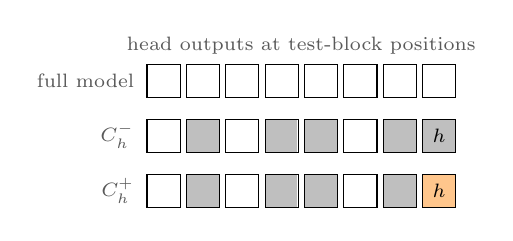
\begin{tikzpicture}[font=\scriptsize,
  head/.style={draw, minimum width=0.42cm, minimum height=0.42cm, inner sep=0pt},
  lab/.style={text=black!65}]
\foreach \r/\name in {0/full model,1/$C_h^-$,2/$C_h^+$} {
  \node[lab, anchor=east] at (-0.25,-\r*0.7) {\name};
  \foreach \i in {0,...,7} {\node[head] (h\r\i) at (\i*0.5,-\r*0.7) {};}
}
\foreach \r in {1,2} {
  \foreach \i in {1,3,4,6} {
    \fill[black!25] ([shift={(-0.2,-0.2)}]h\r\i.center) rectangle ++(0.4,0.4);
  }
}
\fill[black!25] ([shift={(-0.2,-0.2)}]h17.center) rectangle ++(0.4,0.4);
\fill[orange!45] ([shift={(-0.2,-0.2)}]h27.center) rectangle ++(0.4,0.4);
\node at (h17.center) {$h$};
\node at (h27.center) {$h$};
\node[lab] at (1.75,0.45) {head outputs at test-block positions};
\end{tikzpicture}
\caption{Candidate toggle in a fixed retained background. White: live;
grey: role-mean replacement; orange: the candidate restored to live computation.
The two retained configurations differ only in $h$. One is the chosen $C$.
Non-head computation, demonstrations and answer prefixes remain live.}
\label{fig:retained}
\end{figure}

\paragraph{A. Behaviour and background selection.}
On the 20 common families, cross original/swapped mother assignments with the
original/alternative queried child. The cells $x_{00},x_{10},x_{01},x_{11}$ have
gold answers $a,b,b,a$ and retain the fixed $a-b$ scoring sign. Rebuild
tokenization, offsets, masks and the shared answer prefix for changed queries;
do not filter out new-cell errors. For configuration $D$, define
\begin{align}
b_f(D)&=\tfrac14\,\mathbb{E}_o\bigl[
 M_D(x_{00})-M_D(x_{10}) \notag\\
&\hspace{3.7em}{}-M_D(x_{01})+M_D(x_{11})\bigr], \notag\\
B_D&=\mathbb{E}_f b_f(D). \label{eq:bd}
\end{align}
Report the four margins and accuracies, both fact-axis and both query-axis
contrasts, and full-vocabulary first-token outcomes. $B_D$ alone does not establish
correct behaviour in every cell; ratios to the full-model contrast require a
stable denominator.

Evaluate full, empty, $T_1$--$T_5$ and $C_{33}$; evaluate $C_{50}$ only if
$C_{33}$ fails. With
$g_f(D)=\mathbb{E}_o[M_D(x_{00})-M_D(x_{10})]$, the fidelity guards are
\begin{align*}
F(D)&=\frac{\mathbb{E}_f g_f(D)}{\mathbb{E}_f g_f(\mathrm{full})}
       \in[0.8,1.2],\\
L(D)&=\frac{\mathbb{E}_f|g_f(D)-g_f(\mathrm{full})|}
           {\mathbb{E}_f|g_f(\mathrm{full})|}\le0.2,
\end{align*}
with candidate accuracy at most five percentage points below full in every cell
and order separately. Use $C=C_{33}$ if it passes, otherwise $C=C_{50}$; if
both fail, retain $C_{50}$ explicitly as a partial background. If the empty mask
passes, do not claim that the retained heads explain the behaviour. A failed
small-set mask does not disqualify its route from testing inside $C$.

\paragraph{B. Functional participation.}
Evaluate $C_h^-$ and $C_h^+$ for all six candidates on the core four-cell panel,
plus $C\setminus\{\mathrm{L18H19}\}$,
$C\setminus\{\mathrm{L8H15}\}$ and $C\setminus R(C)$.
One state per candidate equals $C$, leaving at most seven distinct candidate
backgrounds. Adding L9H16 to $C_{50}$ gives a 51-head test configuration, not a new
fallback. Record family-level $d_{h,f}=b_f(C_h^+)-b_f(C_h^-)$,
fixed-sign and gold-oriented cell margins, accuracies and changes in $F,L$.
Apply the inherited coherent/heterogeneous rule separately to $d_{h,f}$ and
original-cell gold-oriented margin effects. These tests assess functional
participation in $C$, not membership in a particular route.

\paragraph{C. Association with measured routes.}
Screen all six candidates against all five anchors on the original 40 fact-swap
pairs, in the noising direction. For each state $D=C_h^\pm$,
\begin{align*}
I_{t,f}(D)&=\mathbb{E}_o\bigl[M_D(x_{00})\\
 &\quad{}-M_D(x_{00};t\leftarrow x_{10})\bigr],\\
\gamma_{h,t,f}&=I_{t,f}(C_h^+)-I_{t,f}(C_h^-),
\end{align*}
so $\Gamma_{h,t}=\mathbb{E}_f\gamma_{h,t,f}$ in
Eq.~\ref{eq:ri-route}. Preserve historical route masks, channels and selective
releases. Source donors, frozen increments, receiver captures and fresh recipients
all belong to the same $D$; full-model donors are not reused in retained
backgrounds. Both raw route effects accompany $\Gamma$: a negative difference can
attenuate a positive route or strengthen a negative one. Downstream amplification
can change $\Gamma$ without placing $h$ on the serial path.

A pair is eligible only if the route itself passes the inherited effect rule in
at least one state and its family-level $\gamma$ also passes. Select at most
three pairs: coherent before heterogeneous, then decreasing
$\mathbb{E}_f|\gamma|$, then layer/head and structure ID. A first pass allows
one pair per candidate; a second fills remaining slots with at most two per
candidate. Fill otherwise unused slots only with candidates passing the
functional $d$ rule but having no selected pair, ordered by class,
$\mathbb{E}_f|d|$ and head ID. These receive behavioural follow-up only. Fewer
than three, including zero, is valid; at most three distinct candidates are
selected. Record whether each route-modulation candidate also has a functional
effect. Selection is not revised after reverse patching.

\paragraph{D. Direction and named-connection checks.}
For selected route pairs, repeat the comparison with restoration
$J_t(D)=M_D(x_{10};t\leftarrow x_{00})-M_D(x_{10})$ on the same 40 pairs.
Test one predeclared direct connection per pair
(Table~\ref{tab:final-attachments}) in both directions, alongside a matched
alternative receiver. For each unique connection, sample a receiver from the
same layer, excluding $C_{50}$, all structure members, the original RI set and
the candidate. Freeze controls for every possible connection before new
measurements, using seed 20260926, sorted eligible IDs and lexically ordered
connection keys.

Both the target and control receiver must be live in both compared runs. Thus
these diagnostics use $C_h^+$ plus the control receiver, with the target connection
recomputed in that same background; this differs from the primary modulation
background. V connections use all four fact sentences, excluding question and
colon, without an oracle query-fact restriction; Q connections originate and end
at the colon. Sources precede receivers in layer order; only the receiver's colon
output row is released.

\begin{table}[t]
\centering\scriptsize
\setlength{\tabcolsep}{3pt}
\begin{tabular}{@{}p{1.05cm}p{1.5cm}p{4.55cm}@{}}
\toprule
Structure & Candidate & Direct connection \\
\midrule
$T_1,T_3,T_4$ & $h\in E$ & $h$ / all facts $\to$ L18H18 / V \\
$T_2$ & $h\in E$ except L17H5 & $h$ / all facts $\to$ L16H1 / V \\
$T_2$ & L17H5 & $h$ / colon $\to$ L18H18 / Q \\
$T_1$--$T_4$ & $h\in A$ & L18H18 / colon $\to$ $h$ / Q \\
$T_5$ & $h\in E$ & $h$ / all facts $\to$ L20H1 / V \\
$T_5$ & $h\in A$ & $h$ / colon $\to$ L27H6 / Q \\
\bottomrule
\end{tabular}
\caption{Frozen direct-connection hypotheses.
$E=\{\mathrm{L1H27,L9H16,L11H4,L17H5}\}$ and
$A=\{\mathrm{L23H10,L25H18}\}$.
Shared endpoints do not constitute independent discoveries for each structure.}
\label{tab:final-attachments}
\end{table}

\paragraph{Extension, sensitivity and held-out evaluation.}
On all 89 discovery families, extend only original-query behaviour: full, empty,
$C$, $C\setminus R(C)$ and the additional state of each selected candidate
(at most seven configurations). Repeat the latter retained configurations
(at most five) using the paired opposite-fact donor instead of means,
symmetrically on original and swapped inputs. Report baseline disagreement rather
than selecting the favourable replacement. A fidelity failure leaves $C$ fixed
and labels it partial; it does not trigger another search. New route modulation
and connection checks remain on the 20 common families until validation.

Before the 87 held-out families are opened, freeze $C$, selected candidates and
pairs, controls, expected signs, mean bank, thresholds and input construction.
Validation evaluates the four-cell panel for the same at-most-seven
configurations, selected route modulation in both states and both directions,
selected connections and controls in both directions, and paired-donor
sensitivity. Route and donor tests use the original fact axis only.
Unselected candidates and standalone $T_1$--$T_5$ behaviour remain discovery-only.
Failed validation never triggers replacements or new selection.

\begin{table}[t]
\centering\small
\setlength{\tabcolsep}{3pt}
\begin{tabular}{@{}p{1.2cm}p{1.25cm}p{4.6cm}@{}}
\toprule
Step & Families & Measurements \\
\midrule
A & 20 & Four cells: full, empty, five structures, $C_{33}$; $C_{50}$ only on failure. \\
B & 20 & Four cells: six candidate toggles, two references, collective RI removal. \\
C & 20 & All 30 candidate--route pairs; noising on the original fact axis. \\
D & 20 & At most three selected pairs: restoration; direct connections and controls, both directions. \\
Extension & 89 & Original-query behaviour and paired-donor sensitivity for selected candidates and collective RI removal. \\
Validation & 87 & Frozen four-cell behaviour; selected modulation, connections/controls and donor sensitivity. \\
\bottomrule
\end{tabular}
\caption{Logical order and coverage of the final experiment. Each family has two
fact orders. Functional-only selections omit route and connection tests.}
\label{tab:final-coverage}
\end{table}

\paragraph{Inference and interpretation.}
Average orders within family before aggregating. Report signed and absolute
family effects, each order separately, and mean absolute within-family order
differences. Use 20,000 paired family-bootstrap resamples (seed 20260926);
discovery intervals are descriptive, not selection-adjusted. Apply the inherited
coherent/heterogeneous rule separately to modulation and direct connections in
each direction. A coherent bidirectional result requires coherence in both
directions, the same mean sign, and at least 70\% family sign agreement between
directions. Otherwise report heterogeneity, asymmetry or failure to reproduce.
Report the paired difference in absolute family effects between target connection
and receiver control; without an excess over control, do not claim receiver
selectivity. Its interval is descriptive rather than a new significance test.

Reproduced functional effects and communication support participation in this
task under the declared live background, possibly with an opposing sign. A
functional effect without a retained connection leaves the connection unresolved;
modulation alone leaves overall functional contribution unresolved. A null is
limited to the tested backgrounds, channels and sites. A named connection supports
a link to a member or branch, not exclusive mediation through the whole chain,
and collective RI dependence does not assign a relational role to every member.

\paragraph{Validity checks.}
All-live retention must reproduce the full model, self-donor patches must be
identity interventions in each background, and historical full-model route
anchors must reproduce before new comparisons. Verify structurally zero
no-intermediate fact-to-colon-Q comparators, unchanged earlier fact activations
under query-only edits, identity-free role keys, and live control receivers in
both diagnostic contexts. Input, background, mean-bank population, source/receiver
masks, direction and selective releases must match within every paired contrast.

\subsection{Final-experiment discovery results}
\label{app:s44-results}
The completed run uses the frozen design above: 20 core families, with two orders
and four fact--query cells, followed by the original fact axis on all 89 discovery
families. Its implementation is S45 discovery v2. All numbers here precede the
87-family held-out evaluation reported in Appendix~\ref{app:s44-validation};
the expansion includes the 20 core families.

\paragraph{Retention and order bias.}
All five small sets and both broad sets fail the fidelity guards. Core full-model
gap $g=11.200$ falls to $0.582$ for C33 and $1.283$ for C50; C50 is therefore the
predeclared partial background $C$. Its four-cell contrast is $B_C=0.752$ versus
$5.562$ in full. C50 prefers the first chain's answer candidate in 85\% of the
160 cell--order examples, versus 51.9\% in full, while candidate accuracy is
50\% versus 98.1\%. The original-facts query contrast is $1.497$ versus $10.936$.
The empty-mask core contrasts are zero, although margins vary between families;
its 89-family gap is $0.018$. Retention failure does not locate the missing
computation outside C50 or invalidate routes measured within a richer background.

\paragraph{Individual and collective functional effects.}
Table~\ref{tab:s44-functional} reports core changes in the four-cell contrast.
L9H16 and L1H27 pass coherently, positive in all 20 families. No candidate changes
two-candidate accuracy, although L1H27 increases full-vocabulary top-token
accuracy by five percentage points in two cell--order conditions.
The 31 RI members include eight strong heads; their collective effect does not
isolate the weaker remainder, unlike the S4.2 RI23 comparison.

\begin{table}[t]
\centering\scriptsize
\begin{tabular}{@{}lrl@{}}
\toprule
Head/group & $\Delta B$ & 95\% family interval \\
\midrule
L9H16 & $+0.601$ & $[0.518,0.688]$ \\
L1H27 & $+0.260$ & $[0.215,0.306]$ \\
L11H4 & $+0.004$ & $[0.002,0.006]$ \\
L17H5 & $-0.009$ & $[-0.015,-0.003]$ \\
L23H10 & $+0.004$ & $[0.001,0.007]$ \\
L25H18 & $+0.0003$ & $[-0.004,0.004]$ \\
L18H19 (reference) & $+0.247$ & $[0.197,0.303]$ \\
L8H15 (reference) & $+0.133$ & $[0.103,0.164]$ \\
RI31 jointly & $+0.759$ & $[0.643,0.882]$ \\
\bottomrule
\end{tabular}
\caption{Core functional contributions, 20 families. Intervals are descriptive;
selection follows the predeclared effect rule rather than interval exclusion of zero.}
\label{tab:s44-functional}
\end{table}

\paragraph{Routes and candidate association.}
In C50, T1, T3 and T4 have effects $0.618,0.393,0.255$, retaining 37.2\%, 45.7\%
and 53.4\% of their corresponding full-background core means. T2 and T5 fall
below the rule ($0.042,-0.019$). All 30 candidate--route combinations were
measured; 18 have a retained route in at least one candidate state. None passes
the coherent or heterogeneous modulation rule. The largest mean $\Gamma$ is
L9H16--T1: $+0.0303$ ($[0.0159,0.0464]$); its mean absolute family effect is
$0.0341$, below $0.1$. A small directional interaction is therefore observed,
but no new route association is selected. Only the two functional candidates
advance; the conditional reverse-modulation and attachment tests are not triggered.

A post hoc paired comparison of T1 and T3 isolates the added release of L18H19
alongside L18H18: $+0.225$ ($[0.168,0.283]$) in C50 and $+0.805$
($[0.573,1.055]$) in full, positive in all 20 families. This supports a conditional
contribution of a known RI participant, not an additive share or new candidate
assignment. Below-threshold modulation does not establish that the additional
candidates are outside these routes or act in parallel.

\paragraph{Extension and replacement sensitivity.}
On 89 families, full-model $g=11.170$; C50 retains $1.342$ under means and $2.272$
under opposite-fact donors. Adding L9H16 changes $g$ by $1.210$ or $0.003$;
retaining L1H27 changes it by $0.552$ or $0.006$. Retaining RI31 changes it by
$1.448$ or $4.615$, respectively. These original-axis changes are not the core
four-cell $\Delta B$ values. Under means, C50 gaps are $9.937/-7.253$ by order;
under donors they are $3.141/1.403$. The non-RI remainder under means has gaps
$5.556/-5.767$, cancelling to $-0.106$, rather than being inert. Changing the
baseline changes both the surrounding background and the absent candidate's
replacement; sensitivity alone does not identify redundancy or compensation.

\paragraph{Verification and validation status.}
Independent recomputation reproduced core behaviour, candidate effects and all
1,600 pair-level route records; 1,035 arithmetic and consistency checks passed.
The local extension export contains only the 20 core families, so 89-family
statistics are taken from the frozen summary; their paired intervals were not
independently reconstructed. Figures~\ref{fig:s44-retention-app} and
\ref{fig:s44-effects-app} show the main diagnostics.
The actual frozen validation suite contains six mean configurations on all four
cells and four donor configurations on the original axis, with no selected route
or attachment jobs. Its completed results are reported below.

\begin{figure*}[t]
\centering
\includegraphics[width=0.95\textwidth]{figH_final_retention}
\caption{Final discovery retention and four-cell behaviour on 20 families.
Left: fact-swap gaps with family-bootstrap intervals. Right: fixed-sign margins
by cell and order; correct answers are $a,b,b,a$.}
\label{fig:s44-retention-app}
\end{figure*}

\begin{figure*}[t]
\centering
\includegraphics[width=0.95\textwidth]{figH_final_effects}
\caption{Core functional contributions and candidate--route modulation.
Intervals are descriptive family bootstraps; stars mark routes below retention
in both candidate states. No candidate--route combination passes the effect rule.}
\label{fig:s44-effects-app}
\end{figure*}

\subsection{Final-experiment held-out evaluation}
\label{app:s44-validation}

\paragraph{Frozen scope and verification.}
The completed evaluation uses 87 families disjoint from the 89 discovery
families, with two orders each. The discovery freeze fixes C50 as a partial
background, RI31 and two functional-only candidates, L9H16 and L1H27.
Six mean-replacement configurations cover all four cells; four paired-donor
configurations cover the original fact axis. No candidate--route pair was
selected, so no scientific Gamma or attachment validation was scheduled.
Route probes in the implementation gate are not a route-validation panel.

The completion marker, canonical freeze signature, freeze-file and held-out-plan
hashes, discovery-plan linkage, rosters and code hashes match the frozen run.
Independent recomputation from 522 mean-baseline family records reproduced
state contrasts, fidelity, candidate accuracy, paired effects and bootstrap
intervals; all 226 consistency checks passed. This export includes all eight
cell--order margins for each mean configuration but no donor family vectors,
worker records or mean-bank files. Donor results below therefore use the supplied
87-family summary; no new paired donor intervals are reconstructed. The recorded
gate passed, with zero inert/all-live and earlier-prefix-invariance errors;
maximum clean/corrupted attention reconstruction error was $2.44\times10^{-4}$.

\paragraph{Functional effects reproduce.}
Table~\ref{tab:s44-heldout-functional} contrasts the core discovery effects
with the held-out results. Both candidates pass the frozen coherent rule and
improve the four-cell contrast in every held-out family after averaging orders.
The mean changes by order are $0.592/0.577$ for L9H16 and $0.263/0.259$ for
L1H27; mean gold-oriented margin changes are positive in every cell. The claim
of 87/87 positive families does not mean every family--order effect is positive.
L9H16 raises average two-candidate accuracy from 51.01\% to 53.30\% (16 net
correct decisions over 696 cell--order examples). Retaining L1H27 raises it from
50.57\% to 51.01\% (three net decisions). These accuracy differences are
descriptive; the frozen selection criterion concerns margin contrasts.

\begin{table}[t]
\centering\scriptsize
\setlength{\tabcolsep}{3pt}
\begin{tabular}{@{}lrrl@{}}
\toprule
Head/group & Disc.\ $\Delta B$ & Held-out $\Delta B$ & 95\% interval \\
\midrule
L9H16 & 0.601 & 0.585 & $[0.525,0.656]$ \\
L1H27 & 0.260 & 0.261 & $[0.229,0.301]$ \\
RI31 & 0.759 & 0.727 & $[0.656,0.818]$ \\
\bottomrule
\end{tabular}
\caption{Four-cell contributions under mean replacement: 20 discovery versus
87 held-out families. All three held-out effects are positive in 87/87 families.
Intervals use the frozen 20,000-draw paired family bootstrap.}
\label{tab:s44-heldout-functional}
\end{table}

\paragraph{Replacement dependence also reproduces.}
The original-axis comparisons in Table~\ref{tab:s44-heldout-baselines} use
$\Delta g$, not the four-cell $\Delta B$. Individual candidate effects remain
much smaller under paired-donor replacement. L9H16's mean is near zero and
slightly negative; L1H27's is positive but small. The missing donor family
vectors preclude an independent assessment of donor-effect heterogeneity.
Collective RI31 dependence persists, but includes the eight previously strong
heads and must not be read as validation of RI23 alone.

\begin{table}[t]
\centering\scriptsize
\setlength{\tabcolsep}{3pt}
\begin{tabular}{@{}lrrl@{}}
\toprule
Contribution & Mean $\Delta g$ & Donor $\Delta g$ & Mean 95\% interval \\
\midrule
L9H16 & 1.170 & $-0.002$ & $[1.028,1.345]$ \\
L1H27 & 0.532 & 0.029 & $[0.449,0.633]$ \\
RI31 & 1.404 & 4.427 & $[1.201,1.628]$ \\
\bottomrule
\end{tabular}
\caption{Held-out fact-swap contributions, 87 families. Donor differences are
computed from the supplied configuration means; intervals are reconstructed
only for the mean-baseline paired differences.}
\label{tab:s44-heldout-baselines}
\end{table}

\paragraph{The retained set remains partial.}
Held-out full-model $g=10.918$ and $B=5.433$, versus $g=1.397$ and $B=0.729$
for C50 under means. Candidate accuracy is 98.71\% versus 51.01\%; first-chain
preference is 51.29\% versus 85.49\%. The original-facts query contrast is
$10.899$ versus $1.499$. C50 retains 12.8\% of the fact-swap gap, increasing to
23.5\% with L9H16, still below the fidelity guard. The empty-mask gap is
$-0.013$ and its four-cell contrast $0.002$.

C50 order-specific gaps are $9.820/-7.026$ under means and $2.634/1.213$
under donors; donor fidelity is 17.6\%. Without RI31, its mean-baseline gap
is $-0.007$, but the order-specific values are $5.454/-5.469$: cancellation,
not absence of fact sensitivity. Its four-cell contrast falls to $0.002$.
The corresponding donor gap is $-2.504$ versus $1.923$ with RI31 live.

\paragraph{Outcome labels and interpretation.}
The supplied analyzer labels both candidates ``functional participant,
attachment unresolved''. This label uses mean-baseline functional reproduction;
the label assignment does not incorporate the donor comparisons. We therefore
report reproduced functional participation together with baseline sensitivity,
rather than treating the automatic label as evidence of robustness across
replacement methods. No new threshold or candidate selection is introduced
after validation. The complete-chain measurements, the 30 discovery modulation
contrasts and the post hoc nested-route comparison remain discovery evidence;
the held-out result validates the frozen behavioural comparisons, not new
connections or a sufficient retained circuit.
